\chapter{Evaluation}


In order to define a schema that could hold up to the already defined elements we had to come up with methods that would allow us to quantify and expose valid ways of presenting data. To comply with this, two methods were preselected;  for the evaluation we focused in using a set of predefined conversations that would map to a intent classifier and thus would allow us to quantify the reliability of our intent by using the Accuracy Index of each intent based on the query. This means, that we used the loss function from the model to predict how accurate was the result in comparison to our training phrases and would quantify this by giving a number ranging between 0 - 1, which stands for the percentage of reliability. Moreover, we also defined a second way to quantify our result by preselecting a set of Case Studies that would reassemble a use case of the tool. The idea behind a case study is to quantify the conversation and to give a use case so besides the numerical evaluation we can see how reliable or usable our model is. To introduce the results we will start by describing the quantitative analysis.

\section{Quantitative Analysis}

To have a clear idea of how the loss function works, we must understand the underlying concept in a neural network. As described by Zhao \cite{lossFunction} the loss function is 
\begin{equation}
    \sum \L ^{batch}(sim(a,b), sim(a, b_{1}^{-}),...,sim(a,b_{k}^{-}))
\end{equation}{Described as the loss function from the RASA NLU; where a are the bag of words, b are the labels from the training set, and negative b are extracted from the labels, (a,b) are positive entities of pairs that come from the pretrained set where (a,b) are the pairs. sim() is the similarity function that calculates the inner value using the cosine similarity and finally L denotes the loss function between the positive and negative pairs.}
\begin{figure}[!h]
    \centering
    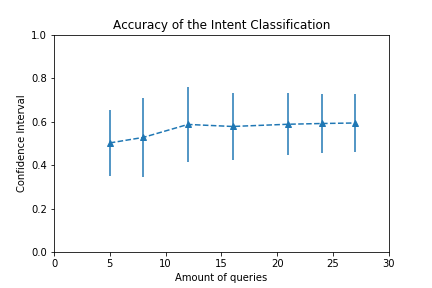
\includegraphics[scale=0.65]{MA-BA-Thesis/AccuracyValidation.png}
    \caption{The Scale of the validation for each user}
    \label{fig:accuracyValidation}
\end{figure}

Thus this would allow us to compute a negative or opposite value for each intent as input in the classifier, meaning that the reminder of the loss function is the accuracy or relative accuracy of the intent classifier result. For each set of values we would have an estimation of the real accuracy level and using this information we could predict the error rate or the relative error rate within the set by using a standard deviation across the group or test set. In order to generate a valid test set we predefined a conversation with the chatbot that could yield the needed results this can be seen in figure \ref{queries_used} where the data was split into several sets. In a first instance all the information coming was split into arrays of queries containing 5, 10, 15, 20, 25, 30 and 35 elements. This elements were selected sequentially and used in different sessions assuming that each conversation was an independent event. Therefore, for each set of conversations we could define a  preset amount of data which in our case ranged from 0.5 to 0.6 meaning a median of 55\% identification rate and classification, even though this might seem like a relatively low identification rate our bot was set to work and accept a yield above 40\% meaning that most of our queries were successfully identified. Despite this, for each case of set of conversation there was an unidentified query or element that was not above the 40\%. Is worth taking into account that the result does not mean that there is a cumulative error since the dataset is unique and thus the errors identified in each stage are transferred to the latter, for example if there was an unidentified intent within the first set, this intent will also appear in the second set since the sets are not unique. The identified error array is as follows:
\begin{table}[!h]
\resizebox{\textwidth}{!}{%
\begin{tabular}{|l|l|l|l|}
\hline
Round Number & Number of Errors( Identification below 40\%) & Rate of Error (\%) & Sample Size \\ \hline
1 & 0 & 0 & 5 \\ \hline
2 & 2 & 20 & 10 \\ \hline
3 & 3 & 20 & 15 \\ \hline
4 & 4 & 20 & 20 \\ \hline
5 & 4 & 16 & 25 \\ \hline
6 & 6 & 20 & 30 \\ \hline
7 & 8 & 22 & 35 \\ \hline
\end{tabular}%
}
\caption{Error in Intent Identification per Round}
\label{tab:intent_classification_error}
\end{table}

Thus, with a round rate of 8/35 in the highest round we could say that the model is acceptable for a beta or alpha release. It's also important to take into account that some of the intents provided in Table \ref{queries_used} contain more than one victim or attack vector and this might lead to errors within the entity identification. Moreover, we can see in Figure \ref{fig:accuracyValidation} that the standard deviation is around 10\% which yield an acceptable value if we refer to a p value of 0.1. Thus, we can say that despite the fact that intent classification is not perfectly achieved, it is still relatively accurate since most intents are mapped within the same context. Whatsoever, it is important to take into detail that the elements in the array are not significantly spread and can give an accurate answer to expand this furthermore we could use this set of intents as additional elements within the validation as training phrases and this would significantly upper our result and most likely all further queries that contain a similar syntax. The intents to benefit the most are the ones with a accuracy rate below 0.4 since they would retrain the transfer model and give us a more significant result in the next iterations. This will be described in the further work section in detail.

Following up, for each set of conversations we received several results that yield from 0 to 8 errors or unidentified intents which in the client side could have a big downstream as the elements that are not directly mapped to an intent just yield an error result. In figure \ref{fig:errorValidation} we can see that the elements that are mapped to each query set produce a high yield of errors but this is relative as they are contained in the previous set. In reality, this sets are meant to match a unique amount of elements not necessarily attached to a group and thus is understandable that the rate varies. Despite this, we must say that an unlikely amount of errors would be around 30\% of the set meaning that more than 11 errors would be a noticeable amount of errors for the tool. Whatsoever, the tool is not featuring learning from the context which can potentially increase the amount of accuracy for intent identification.

\begin{figure}[!h]
    \centering
    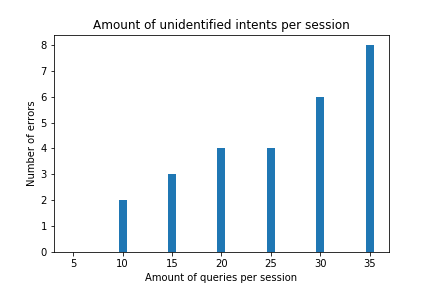
\includegraphics[scale=0.65]{MA-BA-Thesis/ErrorsValidation.png}
    \caption{The amount of errors per each trial session}
    \label{fig:errorValidation}
\end{figure}
To sum up, we can say that the tool can improve in the quantitative area by using the same queries as training phrases and enable the learning from queryng to eventually have a close to perfect model. We do need a supervised training for this whatsoever but this is feasible since the amount of data gathered makes it possible. In order to have a more comprehensive model we must also understand the Case Studies which will give us an idea of the best case scenario for our tool and what to expect out of it, also further improvements can be done in this area.
\begin{table}
\centering
\caption{Queries used for the Evaluation}
\label{queries_used}
\resizebox{\textwidth}{!}{%
\begin{tabular}{|l|l|}
\hline
Number & Example                                                                                                   \\ 
\hline
1      & 'The load balancer graph shows a high increase in traffic'                                                \\ 
\hline
2      & 'The webserver is handling a large amount of packets'                                                     \\ 
\hline
3      & 'The logs show that the router is receiving fragmented packets'                                           \\ 
\hline
4      & 'Seems like there is a smurf atack going on against the memcache servers'                                 \\ 
\hline
5      & 'my ingress controller is getting a lot of DNS responses'                                                 \\ 
\hline
6      & 'Im receiving DNS packets that the server did not request'                                                \\ 
\hline
7      & 'i think im suffering a DNS amplification attack because the servers are getting many DNS answers'        \\ 
\hline
8      & 'the server is getting packets that are too big'                                                          \\ 
\hline
9      & 'the load balancer is getting pings of death'                                                             \\ 
\hline
10     & 'my users are not connecting to the web server because of SYN dissosiation'                               \\ 
\hline
11     & 'my router is getting a huge amount of syn ack packets'                                                   \\ 
\hline
12     & 'the load balancer has low resources and a high amount of fragmented packets'                             \\ 
\hline
13     & 'my web server is getting UDP packets'                                                                    \\ 
\hline
14     & 'the packets on the server are just UDP'                                                                  \\ 
\hline
15     & 'the web server is getting an usual amount of 301'                                                        \\ 
\hline
16     & 'the nginx server gets a lot or redirects 301'                                                            \\ 
\hline
17     & 'the load balancer is prealocating too much memory'                                                       \\ 
\hline
18     & 'the web server is opening several connections at once'                                                   \\ 
\hline
19     & 'the load balancer is opening many connections'                                                           \\ 
\hline
20     & 'the load balancer is recieving a lot of small attacks'                                                   \\ 
\hline
21     & 'my server load is above average'                                                                         \\ 
\hline
22     & 'i cannot access the web server and it is stuck due to high load'                                         \\ 
\hline
23     & 'im getting NTP packets that i didnt request in the server entrypoint'                                    \\ 
\hline
24     & 'Im reciving timestamps that were not requested in my server'                                             \\ 
\hline
25     & 'the server log service shows an usual amount of udp requests'                                            \\ 
\hline
26     & 'i have many open connections in the load balancer and a little bit of data transmited'                   \\ 
\hline
27     & 'I have too many connections right now and the web server is not responsive'                              \\ 
\hline
28     & 'im seeing a very high amount of requests per second in the load balancer'                                \\ 
\hline
29     & 'for some reason the web server is getting a lot of ICMP from other clients'                              \\ 
\hline
30     & 'the apache server has a very high amount of open concurrent connections'                                 \\ 
\hline
31     & 'i see in the logs from the server that the packets are arriving with no information about the protocol'  \\ 
\hline
32     & 'the database server is opening too many sessions'                                                        \\ 
\hline
33     & 'the load of the cluster is very high aparently due to many requests'                                     \\ 
\hline
34     & 'the web server is delivering a lot of ssl certificates'                                                  \\ 
\hline
35     & the web server is getting POST requests with a lot of data'                                               \\
\hline
\end{tabular}
}
\end{table}

\section{Case Studies}

Previously, we defined a quantitative way to define how the model should behave and defined a preset of measures that would yield the desired result. In order to have a different approach to the same set of measurements we decided to come up with use cases that will expand and show how an ideal conversation would give the desired result and how a conversation could contain different elements yet providing a good result. To do this there are two possible routes for a conversation focused towards DDoS attacks that could be useful for the user and for MENTOR. The first set or Case Study will try to reassemble a conversation from top to bottom to generate a solution that could be fitted into mentor and provide a solution. The second case study will reassemble a close to reality conversation that is not necessarily made to fit MENTOR by rather any other kind of recommending system.

\subsection{Case Study \#1 - Requesting for a DDoS protection}

The first case study will try to generate a use-case scenario where a network administrator tries to solve a problem of a DDoS attack by providing a relatively limited amount of data and the chatbot would ask questions accordingly to obtain the most information in each case. Thus. in our first case study we will try to provide elements that can match MENTOR's \cite{recomendationSystem} recommendation algorithm by gathering important elements such as Location, Type of Solution and Budget among other parameters that are needed to generate or classify an optimal solution for a recommending system. Therefore, we can see in Table \ref{tab:case_study1} that the chat bot would query elements to the User and the user would need to answer this questions which certain level of detail. The intents also are described with the accuracy level for each case, thus we can see in the evaluation how close was the intent to the classifier's approximation. Also, is important to say that if an element is missing from the query set such as in the answer number 7 from table \ref{tab:case_study1} we can see that no victim was provided and given a high accuracy rate the chatbot would proceed to ask a followup question to identify the missing entity within the context. At the end of this conversation a JSON file would be generated that would then be fed to MENTOR to generate a solution, the sample of the JSON file can be seen in Listing \ref{lst:json_casestudy} where all the extracted elements are present.

\begin{table}[!h]
\centering
\caption{Case Study 1, the conversation between a user and the chatbot is described as it travels fro the agent from top to bottom. The user queries were entered in a sequential order and the results of the approximations are real and gathered from the evaluator of the conversation.}
\label{tab:case_study1}
\resizebox{\textwidth}{!}{%
\begin{tabular}{|l|l|} 
\hline
ChatBot                                                                                                                                                                & User                                             \\
\hline
\begin{tabular}[c, 10cm]{@{}l@{}}Hi, my name is NetworkBot! I can help you to solve your security issue. \\Try typing something like "I have a high server load." below.\end{tabular} &                                                  \\ 
\hline
(1)                                                                                                                                                                                & Hi                                               \\ 
\hline
Hi! How are you doing?                                                                                                                                                          &                                                  \\ 
\hline
(0.803)                                                                                                                                                                                & i think im under attack                          \\ 
\hline
Can you give me details about the attack                                                                                                                                        &                                                  \\ 
\hline
(0.764)                                                                                                                                                                                & the load balancer is getting fragmented packets  \\ 
\hline
\begin{tabular}[c]{@{}l@{}}So we know that load balancer is having Fragmented Packet right,\\anything else to add?\\\end{tabular}                                               &                                                  \\ 
\hline
(0.578)                                                                                                                                                                                & im getting a lot of pings of death               \\ 
\hline
Can you tell me who was the target?                                                                                                                                             &                                                  \\ 
\hline
(1)                                                                                                                                                                                & the web server                                   \\ 
\hline
\begin{tabular}[c]{@{}l@{}}the web server suffers a and Ping of Death,\\could you provide any other info?\end{tabular}                                                          &                                                  \\ 
\hline
(0.781)                                                                                                                                                                                & no, thats it for now                             \\ 
\hline
Do you need a solution for now or that will work overtime (passive or active)                                                                                                   &                                                  \\ 
\hline
(0.809)                                                                                                                                                                                & an active solution                               \\ 
\hline
where is the target located?                                                                                                                                                    &                                                  \\ 
\hline
(1)                                                                                                                                                                                & in Switzerland                                   \\ 
\hline
How much time do we have for a solution?                                                                                                                                        &                                                  \\ 
\hline
(0.732)                                                                                                                                                                                & within the next hour would be best               \\ 
\hline
For how long should I make the contract?                                                                                                                                        &                                                  \\ 
\hline
(0.486)                                                                                                                                                                                & 3 months is enough                               \\ 
\hline
What is your budget?                                                                                                                                                            &                                                  \\ 
\hline
(1)                                                                                                                                                                                & 4000 swiss francs                                \\ 
\hline
If that is it please type 'that's it for now' and we will prepare a solution                                                                                                    &                                                  \\ 
\hline
(1)                                                                                                                                                                                & that is it for now                               \\ 
\hline
{Ok, sending to MENTOR to generate a solution.}                                                                                               &                                                  \\
\hline
\end{tabular}
}
\end{table}

The Generated JSON File can be used as an input of MENTOR but this will not be covered as the Proof of Concept does not require us to go past the generation of the file. As seen in the JSON file from listing \ref{lst:json_casestudy} the structure reassembles a set of sub-array per each intent; thus allowing most recommending systems to parse based on the identified type and with the specific recommendation. In some particular cases such as currency or duration the sub-elements can also be described as such in arrays within the intent as composite entities.

\begin{lstlisting}[language=json,firstnumber=1,caption={Study Case 1 Generated JSON file}, float, floatplacement=H, label=lst:json_casestudy]
[
   [
      {
         "types_problem":"attack"
      },
      {
         "types_problem.original":"attack"
      }
   ],
   [
      {
         "ddos_attack_chars":"Fragmented Packet"
      },
      {
         "ddos_attack_chars.original":"partial requests"
      },
      {
         "victims":"load balancer"
      },
      {
         "victims.original":"load balancer"
      }
   ],
   [
      {
         "ddos_attack_chars":"Ping of Death"
      },
      {
         "ddos_attack_chars.original":"long pings"
      },
      {
         "victims":"web server"
      },
      {
         "victims.original":"web server"
      }
   ],
   [
      {
         "type_of_service":"proactive"
      },
      {
         "type_of_service.original":"passive"
      }
   ],
   [
      {
         "geo-country.original":"Switzerland"
      },
      {
         "geo-country":"Switzerland"
      }
   ],
   [
      {
         "duration.original":"1 day"
      },
      {
         "duration":{
            "unit":"day",
            "amount":1
         }
      }
   ],
   [
      {
         "duration.original":"3 months"
      }
   ],
   [
      {
         "unit-currency.original":"3000 swiss francs"
      }
   ],
]
\end{lstlisting} 

\subsection{Case Study \#2 - Generic Recommending System and DDoS Attack}
Furthermore, in this case study we aim to provide a generalized solution to the identification of issues, thus we can allow the attack identification intent to gather extra information on each step so the generated JSON file could be fed to another classifier that could predict the solution based on a set of queries. This is done by repeating the process or gathering as much information possible from the attack identifier intent.

The idea behind the second case study is to find which is the easiest method to gather information from the user without having to preset limitations on normal constraints in contrast to case study 1 where the elements where extracted to fit MENTOR \cite{recomendationSystem} with the benefits that would allow to gather more information and thus retrain the machine learning model to allow a constant expansion on the information obtained. Moreover, the model only obtains information extracted from intents; as an extension a heading or key can be added to detect the intent from which it comes from with the idea that it can be extracted from any tool by just reading the header of each element, similar to how frontend systems parse responses from backend systems. 

Its important to say that despite the fact that the conversation was shorter, the JSON file can grow to several lines as the identification of the intent grows. The only way this can be limited is if the file is not mapping the right intents. As a current limitation if there is a disruption of the conversation and there is not fallback intent then the system restarts to the beginning.

\begin{table}[!h]
\centering
\caption{Case Study 2 Chat Demo}
\label{tab:casestudy2}
\resizebox{\textwidth}{!}{%
\begin{tabular}{|l|l|} 
\hline
ChatBot                                                                                                                                                                         & User                                                                                                                              \\ 
\hline
\begin{tabular}[c]{@{}l@{}}Hi, my name is NetworkBot! I can help you to solve your security issue. \\Try typing something like "I have a high server load." below.\end{tabular} &                                                                                                                                   \\ 
\hline
(1)                                                                                                                                                                                & Hi                                                                                                                                \\ 
\hline
Hi! How are you doing?                                                                                                                                                          &                                                                                                                                   \\ 
\hline
(1)                                                                                                                                                                                & im suffering an attack                                                                                                            \\ 
\hline
Can you give me details about the attack                                                                                                                                        &                                                                                                                                   \\ 
\hline
(0.790)                                                                                                                                                                                & the web server is only getting partial requests                                                                                   \\ 
\hline
\begin{tabular}[c]{@{}l@{}}the web server suffers Fragmented Packet, \\could you provide any other info?anything else to add?\end{tabular}                                      &                                                                                                                                   \\ 
\hline
(0.77)                                                                                                                                                                                & \begin{tabular}[c]{@{}l@{}}also the database server is receiving a \\high number of request a lot of pings of death\end{tabular}  \\ 
\hline
\begin{tabular}[c]{@{}l@{}}the database server suffers High number of request,\\~could you provide any other info?\end{tabular}                                                 &                                                                                                                                   \\ 
\hline
(0.704)                                                                                                                                                                                & also, i have low resources                                                                                                        \\ 
\hline
and what is the target?                                                                                                                                                         &                                                                                                                                   \\ 
\hline
(0.714)                                                                                                                                                                                & the main server                                                                                                                   \\ 
\hline
\begin{tabular}[c]{@{}l@{}}So we know that also is having Low Resources \\in the main server right, anything else to add?\end{tabular}                                          &                                                                                                                                   \\ 
\hline
(0.656)                                                                                                                                                                                & end here                                                                                                                          \\ 
\hline
\begin{tabular}[c]{@{}l@{}}Ok, Generating JSON File with the obtained values.\\~Mentor won't be able to use them thought.\end{tabular}                                          &                                                                                                                                   \\
\hline
\end{tabular}
}
\end{table}

As observed in table \ref{tab:casestudy2} each element maps to the input from the query on the right side. Below each response form the chatbot there is a number which denotes the confidence level of the intent classifier; meaning that in general the generic intent identifier has a higher success rate than the case study 1 which is tailored to fit a recomending system. This is expected since the chatbot was tweaked to fit the intent classifiers of common DDoS attacks rather than other sets of questions such as location or currency.
\subsection{Analysis from evaluation}

We can sum up the case studies by denoting that most of the intents have a relatively high amount of positives which denote a good level of accuracy for both models. It us important to contrast both in order to understand how a tailored solution can be made using the same model and just modifying the set of intents to be queried. In the case of the study 1 we aimed for a more explicit and templated set of answers which usually will reduce the amount of errors through the process. Meanwhile, the second case study presents a more general an usable use case but sacrifices the areas where data could be erroneously interpreted. 

In order to get the best of both worlds in an ideal representation or production case we should aim to use both the generic model but tailored with modifications to fit the recommending system to avoid the chatbot generating errors or miss-interpreting the input. Needless to say that the chatbot classifier could also gather an input with a confidence interval higher than 40\% and thus saiving to the JSON file an element which might not be an accurate representation of the intent. For our first case study we used a bigger set of intents which is prone to more errors from one side but also easier to debug and to add fallback methods as the granularity of the solution increases in a controlled environment. On the other side, it is hard to predict the granularity based just on the input, the only way to guarantee this is by increasing the amount of training phrases to include high and low granularities or to decide the granularity by questions such as in the first case study.

\begin{figure}
    \centering
    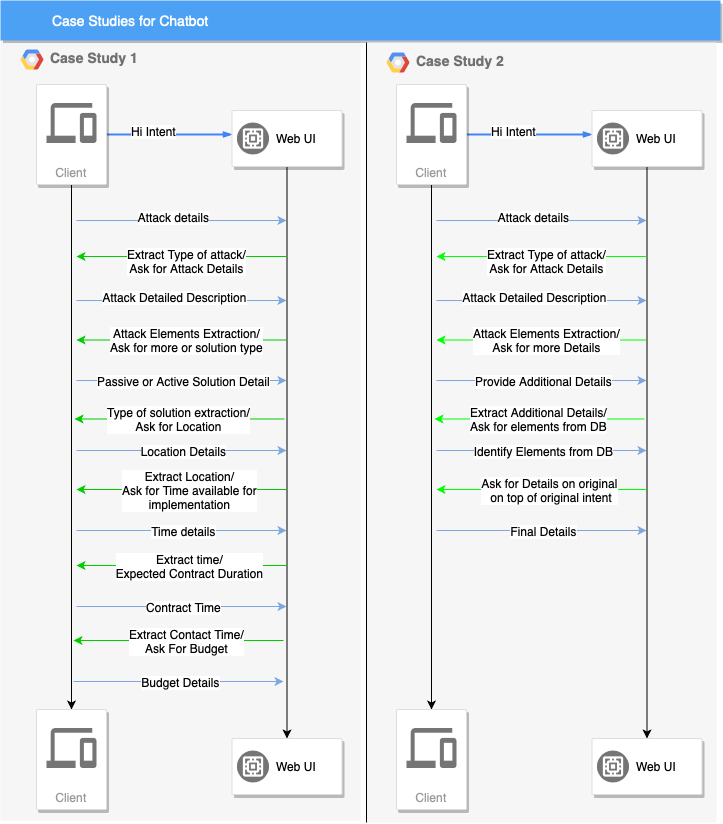
\includegraphics[scale=0.53]{MA-BA-Thesis/CaseStudies.png}
    \caption{Case Studies Comparison Graph, Case study 1 from top to bottom on the left side, Case study 2, right on the right side.}
    \label{fig:case_studies_comparison}
\end{figure}{}


\begin{lstlisting}[language=json,firstnumber=1,caption={Case Study 2, Generic Requirement Gathering}, float, floatplacement=H, label=lst:json_casestudy2]
[
   [
      {
         "types_problem":"attack"
      },
      {
         "types_problem.original":"attack"
      }
   ],
   [
      {
         "victims":"load balancer"
      },
      {
         "victims.original":"load balancer"
      },
      {
         "ddos_attack_chars":"SYN Flood"
      },
      {
         "ddos_attack_chars.original":"SYN packets"
      }
   ],
   [
      {
         "ddos_attack_chars":"Low Resources"
      },
      {
         "ddos_attack_chars.original":"low resources"
      },
      {
         "victims":"web server"
      },
      {
         "victims.original":"web server"
      }
   ],
   [
      {
         "victims.original":"database"
      },
      {
         "ddos_attack_chars":"many NTP results"
      },
      {
         "ddos_attack_chars.original":"many NTP results"
      },
      {
         "victims":"database server"
      }
   ],
   [
      {
         "victims.original":"database"
      },
      {
         "ddos_attack_chars":"many NTP results"
      },
      {
         "ddos_attack_chars.original":"many NTP results"
      },
      {
         "victims":"database server"
      }
   ]
]
\end{lstlisting} 

\section{Discussion}

Among very important areas discussed throughout the previous chapters, is relevant to tackle areas that could be improved and that are not necessarily defined as there is room for improvement or merely choice. This is the case starting from the beginning with areas such as NLP which is show to be beneficial compared to traditional methods of looking for a particular word in a context from a provided bag of words
\cite{nlpComparisson} despite this, we can not say that this would solve the problem of interpretation within the context; Moreover as shown by Duran \cite{nlpComparisson} the are several limitations between traditional methods and NLP classifiers such as expressions proper to the language that could affect the way in which words can be recognized. For example a computer can be male or female in french and also could mean a different thing depending on the context, therefore traditional options are not always the answer.

Moving forward to another aspect which is the tool set for the Machine Learning algorithms to be trained into is a topic worth being discussed. As described in Chapter 3 the best choice for our chatbot was Google Dialog Flow in contrast to other tools such as Microsoft's LUIS or IBM's Watson, despite this there are interesting areas were we could presume that our assumption was not completely valid. Despite the fact that we can use DialogFlow composite entities, in practice this entities could have been used better in conjunction with a preset intent classifier. After gathering enough data the best way to continue the development of the tool would be to use a Supervised Embedding classifier instead of using a pre-trained model with transfer learning. This is detailed by Gardner \cite{spacy} and in comparison the supervised model was rerun under a Recurrent Neural Network resulting in more accurate classifiers using less information.This is set to test and trial but is strictly related to the fact that this is not possible in DialogFlow and thus would have to be used in RASA which features an open implementation. This is also further expanded by the classifier and could be targeted using interactive learning from the RASA core which expands datasets using an algorithm similar to CBOW from Mikelov \cite{word2vec}. Also, related to the NER extraction we are limited to DialogFlow's pretrained extractor, for our base case this is fine as having a custom entity recognition component would be out of scope but is worth taking into account, whatsoever this will be expanded on the further work section. Is worth mentioning that if we wanted to keep the implementation open source there was the chance to implement composite entities using RASA from Sklearn and tokernizer pipeline, albeit this was out of scope as the implementation would have taken more time that the given for this project. Other options that could also be named is Wit.Ai which provides an API for automated intent recognition with the underlying technology of RASA but tweaked using pretrained models, similar to DialogFlow

Another important aspect that is worth analysing is the API being used from DialogFlow, which is at the moment the version number two but is prone to changes. This happened during the development of the the chatbot, were Google announced a change from the API V1 to V2 and the first version was being phased out. Despite this being a not necessarily disruptive behavior in order to maintain and have a long lasting solution we must opt to use a service that is not maintained/updated by third parties. This opens the lead to a few other cases for example when is the best time to swap technologies and for how long can a chatbot run in legacy mode; all these issues are related to having the server running at a external thus using an opensource alternative such as RASA might yield a better result if we aim to have a long lasting self maintained application. Likewise, if we want to have a reliable system which should be up to date periodically the preferred option should be DialogFlow. During the process of enabling authentication for V2, several issues rose such as the need for a server side application that could handle the authentication to avoid client side authentication directly with the DialogFlow API. To prevent this, we developed a client that only runs in the server side of the application when the application is served generating the tokens, whatsoever this implementation is not ideal as the authentication tokens had to be hardcoded into the code and the login mechanism generates a token and a refresh token for each login. This is not an ideal situation and also prevents using security metrics such as requests per login.

Other aspect that is quite relevant for the development and further expansion of the chatbot is the granularity of the use. This is very important since the development of the chatbot goes strictly related to the usage and the target user of a chatbot. Lets take for example an Airplane company and its users who will most likely have simple questions related to flights and customer support, when a question becomes to complex a human will have to intervene. This is because of the granularity of the problem, different use cases have different levels of granularity. To put it in perspective for our chatbot we can take for example a simple issue with a very low granularity such as "my computer is slow" vs an issue with a quite high granularity such as "my web server is running nginx and the logs show that the handler has connections that are kept alive over 5000 ms thus depleting the resources of the node", given this two examples we can see that the difference in granularity plays a key role and despite the fact that we could ask the user to input the level of granularity to be used this could be more prejudicial than beneficial. Overtime, this issue can be overcome using a supervised learning model that takes this into account and with enough information is capable of creating a subset of intent classifiers. Whether this solution will be used in practice by more expert users is prone to evaluation since most advanced users expressed the lack of need to use external tools to solve common day issues as described by Botta \cite{usageSecurity}.

During the Approach we stumbled upon many interesting aspects that can be found relevant was the usage of the extracted data. For our proof of concept the extracted data was not fully used as we decided to focus only in the DDoS section and most of the extracted information that lies within is subject to reprocessing. Within the chatbot code the functions for tool assessment and recommendation are available using the information obtained from the database, whatsoever for the DDoS attack intents this information is barely used as there is not much information about DDoS attacks within the UNIX man-page tool-set and thus if we would like to expand our chat bot to map recommendations related to unix manpage this is feasible by doing some changes to the existing model or by just extending the current model.

Among the development of the intents and the entity map its clear that there are methods that could provide a better result in terms of performance or at least result in a higher confidence interval, now the trade off would be to have additional information from a single source and then train expecting a higher confidence interval than with the established model. Now, this could have to results since we would be expanding both the intent and the entities using NLP rather than NLU so we could possibly have a higher amount of fake positives than we should have. Meaning that we would have a higher confidence interval but the result from this classifier would match to an intent that does not relate to the user need. Therefore, we are limited in this way by the amount of intents at least that can be created because this most be supervised instead of a traditional unsupervised learning, this is interesting because new methods of how to map embeddings in NLU are becoming a trend such as using LSTM as defined by Young \cite{NLP_LTSM} by combining a multiplier of inferences to have long term short memory instead of passing contexts through a pipeline. Is posisble that this will become the default in the coming years but at the moment opensource chatbots that have a pretrained pipeline such as RASA use SVM as a defacto since RASA does not create the word embeddings.

Also, an interesting aspect regarding the process of extraction is related on the storage of the information. Since the base was a postgresql database we decided to stick to this one, but it seems like having everything in a nosql database such as DataStore is way better as we have no need of relationships and the insertions are rather rare in comparison to the readings. This was described in the paper by Padhy \cite{nosql} where we can see that in some cases noSQL Databases have a better performance when there are not too many columns and thus in our particular case once the index is built there is no need for a relational database. Moreover, the extraction of the data used the name, short name, synopsis and description. These elements are not standardized and thus not all of them can be used for example the description, is up to the usage and the project to implement this or not but in our case the description was no necessary. Following up on this, the structure definition was very close to our goal and the model seem to reassemble very close to common problems in the space of identifying key factors in the area of DDoS attacks, furthermore changes would be needed to adapt this to other use cases.

The overall section that features fullfilment describes a brief implementation of the system controller, sadly this is not a complete picture of how the control of the information flows. While using cloud functions might sound very appealing we are also bound to the vector and thus in order to avoid using this function we would have to jump to another function service provider such as AWS Lambda. Despite the fact that there are open source alternatives such as open faas, the implementation still remains a milestone to solve. Moreover, related to this is the fact that we trained our model only using positive training phrases that reassemble the expected intent, whatsoever we did not feed negative examples of what is not what the intent look like, this is because of a time constraint and to certain extent is not needed unless there are two intents which are quite similar and we need to dissociate one from the other.

The architecture is also prone to improvement and discussion as many of the elements provided in the architecture are highly bound to google cloud platform, for example the client authentication. If we wanted to escape vendor lock then the best way would be to avoid using google data store and dialogflow and replace them with RASA and a database such as MongoDB plus a open ML pipeline that can feature options such as automated training and management of data. This is again relevant to the project and the implementation. Once again, this is also related to the content that can be fed into the algorithms, if possible we would like to use a big amount of data but if this is not feasible then a pretrained model would be the best approximation.

The User interface works in a quite simple manner and would say that is quite successful, moving the authentication to a server side and reuse tokens is feasible but would raise questions regarding security. Even though this is a trade off, we can rework the login algorithm to perform the login operation faster. As for the responses, DialogFlow can feature a set of additional options that can be included and expanded on the model on the fly. Meaning that we could support voice to text or custom intents within the model to perform certain actions based on the input, for example we could open a browser with google to look for certain term after the bot would extract certain elements from the conversation that map to obvious solution, now we do not know if this would be beneficial for the user or a distraction, thus is prone to usage depending on the application. In our case this does not make sense as we want to gather as much information as possible from the user.

\subsection{Threats to Validity}

There are many areas where we have to limit the scope of the research and take into account that not all the changes were supposed to aim for a single objective which is having a functional working client that can solve issues related to DDoS attacks. In a general case this is not a problem as this solution can be expanded into other interesting areas such as tooling and problem resolution within the operating system. What so ever we must take into account some aspects that we assumed under ideal scenarios but would not scale in other scenarios. 

Lets take for example the intent classifier which is currently looking for two key elements which is a symptom within the the attack that could be between a very simple issue with resources or a very complex problem that has to do with the frames within the packets. For our solution we assumed a median case scenario where the problem is properly described, in order to get more detailed information for the user a more detail model would need to be implemented by increasing the amount of intents. Even though this is not impossible, certainly would take much more time and will not have a big impact in the generic behavior of the chatbot.

Another limitation in our project is the intent classifiers themselves as for each we have to provide a set of training phrases that have to be specific for each kind of usage. If we try to take into account a different set of training models instead of a supervised trained model but rather a recurrent neural network that features reinforcement learning we could save time and let the algorithm retrain on each iteration. What so ever, we are limited in our case because DialogFlow is the owner of the code and to train in this particular way we would need to migrate the setup to an open source solution such as RASA or create custom datasets that could reassemble the training process using Google's natural language notebooks.

Additionally, the model takes into account predefined entities. Even though, we extracted over 300 entities form the manned DB a secondary manual inspection was also needed and this could raise issues if we decide to automate the process of reinsertion of the data. Worth mentioning that if we can reach an average confidence interval of 50\% then we could potentially say that above 55\% we can reinsert the data into the database and learn from this. Now this is a limitation of the dataset we picked. Alongside, the context can include a limited amount of information and the number of intents to which the context can be passed to is also limited and this is predefined by DialogFlow which specifies that for each intent we can only pass the element to the next 5 intents. This is a limitation that lies within LSTM ( Long Short Term Memory) and the way the recurrent network spreads and retrains.

Finally, we have to assume that the model works using positive examples, as we did not include any negative phrases to avoid collisions in the model, meaning that is possible that there is not a major improvement using negative phrases and if there is we would need to include these negative phrases manually as they are only available in the model trainer but not in the UI that the user has access to. This continues since most of our limitations lie within the DialogFlow capabilities particularly in the NER extractor and the training of the intent classifier, in order to avoid this we would need to migrate the model to RASA.


